\documentclass{article}


% if you need to pass options to natbib, use, e.g.:
%     \PassOptionsToPackage{numbers, compress}{natbib}
% before loading neurips_2022


% ready for submission
\usepackage[preprint]{neurips_2022}


% to compile a preprint version, e.g., for submission to arXiv, add add the
% [preprint] option:
%     \usepackage[preprint]{neurips_2022}


% to compile a camera-ready version, add the [final] option, e.g.:
%     \usepackage[final]{neurips_2022}


% to avoid loading the natbib package, add option nonatbib:
%    \usepackage[nonatbib]{neurips_2022}


\usepackage[utf8]{inputenc} % allow utf-8 input
\usepackage[T1]{fontenc}    % use 8-bit T1 fonts
\usepackage{hyperref}       % hyperlinks
\usepackage{url}            % simple URL typesetting
\usepackage{booktabs}       % professional-quality tables
\usepackage{amsfonts}       % blackboard math symbols
\usepackage{nicefrac}       % compact symbols for 1/2, etc.
\usepackage{microtype}      % microtypography
\usepackage{xcolor}         % colors

% Felix's packages
\usepackage{todonotes}
\usepackage{amsmath}
\usepackage{amssymb}
\usepackage[shortlabels]{enumitem}
\usepackage{mathtools}
\usepackage{mathrsfs}
\usepackage{dsfont}
\usepackage{physics}
\usepackage{caption}
\usepackage{subcaption}
\usepackage[nameinlink]{cleveref}
\usepackage{float}

% floor, ceiling, set
\DeclarePairedDelimiter{\ceil}{\lceil}{\rceil}
\DeclarePairedDelimiter{\floor}{\lfloor}{\rfloor}
\DeclarePairedDelimiter{\set}{\lbrace}{\rbrace}
\DeclarePairedDelimiter{\iprod}{\langle}{\rangle}
\DeclarePairedDelimiter{\card}{\lvert}{\rvert}
\let\abs\relax
\DeclarePairedDelimiter{\abs}{\lvert}{\rvert}
\DeclarePairedDelimiter{\level}{\llbracket}{\rrbracket}

\DeclareMathOperator{\Int}{int}
\DeclareMathOperator{\bdy}{bdy}
\DeclareMathOperator{\Lim}{Lim}
\DeclareMathOperator{\mean}{mean}
\DeclareMathOperator{\col}{col}
\DeclareMathOperator{\proj}{proj}
\DeclareMathOperator{\dual}{dual}
\usepackage[nameinlink]{cleveref}
\DeclareMathOperator{\opt}{opt}
\DeclareMathOperator{\cone}{cone}
\DeclareMathOperator{\conv}{conv}
\DeclareMathOperator{\supp}{supp}
\DeclareMathOperator{\poly}{poly}
\DeclareMathOperator{\sgn}{sgn}
\DeclareMathOperator{\depth}{depth}
\DeclareMathOperator{\OPT}{OPT}
\DeclareMathOperator{\Set}{set}
\DeclareMathOperator{\pred}{pred}
\DeclareMathOperator{\SAT}{SAT}
\DeclareMathOperator{\indeg}{indeg}
\DeclareMathOperator{\outdeg}{outdeg}
\DeclareMathOperator{\tw}{tw}
\DeclareMathOperator{\bw}{bw}
\DeclareMathOperator{\pw}{pw}
\DeclareMathOperator{\cutwidth}{cutwidth}
\DeclareMathOperator{\Cut}{Cut}
\DeclareMathOperator{\Vs}{Vs}
\DeclareMathOperator{\vs}{vs}
\DeclareMathOperator{\adj}{adj}
\DeclareMathOperator{\Sp}{Sp}
\DeclareMathOperator{\argmax}{argmax}
\DeclareMathOperator{\argmin}{argmin}
\DeclareMathOperator{\dom}{dom}
\DeclareMathOperator{\MLE}{MLE}
\DeclareMathOperator{\MAP}{MAP}
\DeclareMathOperator{\KL}{KL}
\DeclareMathOperator{\LK}{LK}
\DeclareMathOperator{\Be}{Be}
\DeclareMathOperator{\Bin}{Bin}
\DeclareMathOperator{\Geo}{Geo}
\DeclareMathOperator{\Po}{Po}
\DeclareMathOperator{\Exp}{Exp}
\DeclareMathOperator{\Mult}{Mult}
\DeclareMathOperator{\Var}{Var}
\DeclareMathOperator{\Cov}{Cov}
\DeclareMathOperator{\Cauchy}{Cauchy}

% commonly used sets
\newcommand{\R}{\mathbb{R}}
\newcommand{\Z}{\mathbb{Z}}
\newcommand{\N}{\mathbb{N}}
\newcommand{\Q}{\mathbb{Q}}
\newcommand{\C}{\mathbb{C}}
\newcommand{\E}{\mathbb{E}}
\newcommand{\B}{\mathcal{B}}
\newcommand{\F}{\mathcal{F}}
\renewcommand{\L}{\mathcal{L}}
\renewcommand{\P}{\mathbb{P}}

\newcommand{\sset}{\subseteq}
\newcommand{\mcal}{\mathcal}
\newcommand{\mscr}{\mathscr}
\newcommand{\mfrak}{\mathfrak}
\newcommand{\up}{\uparrow}
\newcommand{\down}{\downarrow}
\newcommand{\zeros}{\mathds{0}}
\newcommand{\ones}{\mathds{1}}
\newcommand{\tends}[1]{\xrightarrow{#1}}

\newcommand{\Partition}{{\sc Partition}}

\renewcommand{\bibsection}{}


\title{Weighted Maximum Independent Set Heuristics with Graph Neural Networks}


% The \author macro works with any number of authors. There are two commands
% used to separate the names and addresses of multiple authors: \And and \AND.
%
% Using \And between authors leaves it to LaTeX to determine where to break the
% lines. Using \AND forces a line break at that point. So, if LaTeX puts 3 of 4
% authors names on the first line, and the last on the second line, try using
% \AND instead of \And before the third author name.


\author{%
  Felix Zhou\\
  Department of Computer Science\\
  Yale University\\
  New Haven, CT 06511 \\
  \texttt{felix.zhou@yale.edu} \\
  % examples of more authors
  % \And
  % Coauthor \\
  % Affiliation \\
  % Address \\
  % \texttt{email} \\
  % \AND
  % Coauthor \\
  % Affiliation \\
  % Address \\
  % \texttt{email} \\
  % \And
  % Coauthor \\
  % Affiliation \\
  % Address \\
  % \texttt{email} \\
  % \And
  % Coauthor \\
  % Affiliation \\
  % Address \\
  % \texttt{email} \\
}


\begin{document}


\maketitle


\begin{abstract}
  The weighted maximum indepedent set (WMIS) problem asks us to find a subset of pairwise non-adjacent vertices
  which maximizes the sum of vertex weights.
  In general, there cannot be a constant factor polynomial time approximation algorithm.
  In theory, much progress has been made for solving WMIS for special classes of graphs.
  In practice, exact algorithms based on reduction rules and branching techniques have been examined
  in conjunction with search-based heuristics.
  Graph neural networks (GNNs) have been shown to be effective at learning the structure of real-world graphs.
  Recent efforts have been made to combine simple GNNs with exact methods and iterative search.
  We analyze the performance of GNN architectures within this paradigm.
  We also provide an easily extensible python implementation of our algorithms for futher exploration.
\end{abstract}


\section{Introduction \& Problem Definition}
Let $G=(V, E)$ be a (simple, undirected) graph with vertex set $V$
and edge set $E$.
Suppose we also have vertex weights $w: V\to \R_{++}$.
Recall that a subset of vertices $I\sset V$ is \emph{independent}
if for every $u\neq v\in I$, $uv\notin E$.
That is, the vertices in $I$ are pairwise non-adjacent.
The weighted maximum independent set problem (WMIS)
asks us to find an independent set $I$ which maximizes $w(I) := \sum_{v\in I} w(v)$.
Note that $I$ is a WMIS in $G$
if and only if $V\setminus I$ is a weighted minimum vertex cover (WMVC) in $G$.
The unweighted decision version of the minimum vertex cover problem (MVC)
was one of Karp's original 21 NP-complete problems.
It follows that both WMVC and WMIS are both NP-hard.
In general graphs,
it is known that the independent set problem (MIS) cannot be approximated within a factor of $n^{1-\epsilon}$ for any $\epsilon > 0$ where $n$ is the number of vertices \citet{zuckerman2006linear}.
In fact, even in 3-regular 3-edge-colorable graphs,
there can be no polynomial time approximation scheme (PTAS) \citet{berman1999appr}.

\section{Overview of Results}
We trained two simple GNN models,
BASELINE and WMVC which both consist of three message passing layers
interwoven with 3-layer MLPs.
The main difference is the addition of a graph attention convolution \citet{brody2021attentive},
a spectral convolution \citet{defferrard2016conv},
and multiple aggregation heads \citet{corso2020principal, tailor2021we} in WMVC which BASELINE lacks.

We also implemented a simple reduction step which involves solving a single linear program
as well as a simple greedy postprocessing step to round the output probabilities on each vertex to an integral solution.
This heuristic is quite modular and any of the three components
(reduction, GNN, postprocessing)
can be replaced with more sophisticated implementations.
We discuss possible directions of improvement in each of the three components
within \Cref{sec:conclusion}.

Our experiments show that GNNs are able to learn some inherent structure of large independent sets
and were able to generalize to unseen examples,
even ones which contain significantly more nodes than the training examples.
This is quantified in the quality of approximations our extremely simple heuristic was able to achieve.

\section{Related Works}
\subsection{Reductions}
It is helpful to think of WMIS as a 0-1 integer program.
\begin{align*}
  &\max \sum_{v\in V} w(v) x(v) \\
  x(u) + x(v) &\leq 1 &&\forall uv\in E \\
  x &\in \set{0, 1}
\end{align*}
Although we cannot hope to solve 0-1 integer programs in polynomial time
(unless P=NP),
we can relax the integral constraints ($x\in \set{0, 1}^n$)
to form a linear program ($x\in [0, 1]^n$).
Solving this linear program yields a solution $\bar x\in [0, 1]^n$.
It is known that there is an optimal solution to WMIS
such that if $\bar x(v) = 1$,
then the solution includes $v$
and if $\bar x(v) = 0$,
then the solution does not include $v$ \citet{lpreduction}.
Thus we can shrink an instance of WMIS by first solving a linear program
and enforcing that integral vertices are (not) part of the solution.
This is an example of a reduction rule
which reduces the sizes of instances
such that any optimal solution for the reduced instance can be expanded to an optimal solution
for the original solution.
Practical solvers for WMIS extensively use reduction rules
in hopes that we can significantly reduce instances
before applying brute force or a heuristic search \cite{kamis}.

We employ the simple LP reduction rule by calling upon the popular LP solver Gurobi \citet{gurobi}.
Using this simple reduction rule allows ease of implementation in python
as well as delegate the heavy lifting to a library.
While reduction rules with better practical performance are known and implemented in C++,
it would be difficult to integrate with existing machine learning pipelines.

\subsection{Graph Neural Networks}
Graph neural networks generalize the concept of convolutions
within convolutional neural networks
to arbitrary graph-structured data \citet{scarselli2008graph}.
Neural network architectures for graphs have made non-trivial progress on combinatorial optimization problems \citet{cappart2021combinatorial}.
For example, we can consult a graph convolutional network (GCN) as part of an iterative search,
whether some vertex is part of some optimal solution \citet{comboptgcn}.
The authors referred this as a \emph{reducing-peeling} strategy.

Following this line of works,
\citet{langedal_et_al} combined techniques from exact methods,
iterative search,
and GNNs.
The authors first compute a greedy solution using reduction rules when possible.
Then, a GNN is applied to select a vertex likely to be in or out of the solution,
potentially opening up further reductions.
Finally, a local search strategy is used to enhance the solution.
They also provided a C++ implementation
and conducted experiments on some SuiteSparse graphs \citet{suitesparse}.
However, we were unable to obtain the exact dataset used.

We focus our experimentation on the GNN aspect of the heuristc from \citet{langedal_et_al}
and less on the reduction rules and postprocessing step.
Moreover, our implementation fits well into the broader data science landscape around python
and lends itself towards future research directions.

\subsection{Unsupervised Techniques}
Data preparation is an important component of any machine learning pipeline.
One of the many bottlenecks in supervised learning is obtaining labelled data.
This hurdle is even more apparent in our setting
since it is NP-hard to produce the exact labels for an optimal solution.
Moreover, even if we do manage to optimally solve a sufficient number of instances
to produce a sizeable training set,
there is no guarantee that these solutions are unique.
\citet{karalias2022neural} take a different route
and bypass the labelling by extending discrete functions onto a continuous domain
and directly training a GNN to optimize these functions.
This follows an extensive line of work for gradient progagation
through discrete functions \citet{williams1992simple,bengio2013estimating,karalias2020erdos}.

These unsupervised techniques provide an alternative to the training of the GNN
and perhaps unlock training at larger scales than what we have been able to accomplish.

\section{Our Approach}
Our approach can be summarize by the following:
\begin{enumerate}[1)]
  \item Compute reductions (optional).
  \item Consult GNN as in reducing-peeling.
  \item Go to 1) (optional).
  \item Compute a final feasible solution.
\end{enumerate}
Our overall goal is two-fold.
First, we would like to build on the framework of \citet{langedal_et_al}
with a focus on the architecture of the GNN employed
and less attention on the reductions and local search techniques.
Secondly, we would like to provide a highly extensible framework in Python3
which faciliates further experimentation.

\subsection{Computing Reductions (Optional)}
Before consulting our GNN,
we can optionally apply some reduction rules.
We will leverage the popular LP solver Gurobi \citet{gurobi}
and implement the LP reduction by \citet{lpreduction}.

Other reduction rules which we have not implemented include
neighborhood removal,
where a vertex is swapped into a solution if its neighbors have sufficient weight,
weighted twin,
where two vertices with the same independent neighborhood can at times be directly included into the solution,
and weighted domination,
where if vertices $u, v$ satisfy $N(u)\cup \set{u} \supseteq N(v)\cup \set{v}$,
but $w(u) < w(v)$,
then $u$ can be removed \citet{kamis}.
These reductions can all be implemented and swapped or added to the reduction step of our algorithm.
However,
a sufficiently fast implementation would be difficult in python.
Thus we leave the experimentation with more complex reduction rules for future work.

\subsection{GNN Architecture}
\subsubsection{BASELINE}
We first implement the 3-layer GNN architecture from \citet{langedal_et_al}
implemented in PyTorch Geometric \citet{pyg},
a library built upon the popular PyTorch framework \citet{pytorch}.
We refer to this model as BASELINE.
It consists of three message passing layers
interwoven with 3-layer MLPs
as well as a random walk positional encoding \citet{dwivedi2021graph}.

\begin{figure}
     \centering
     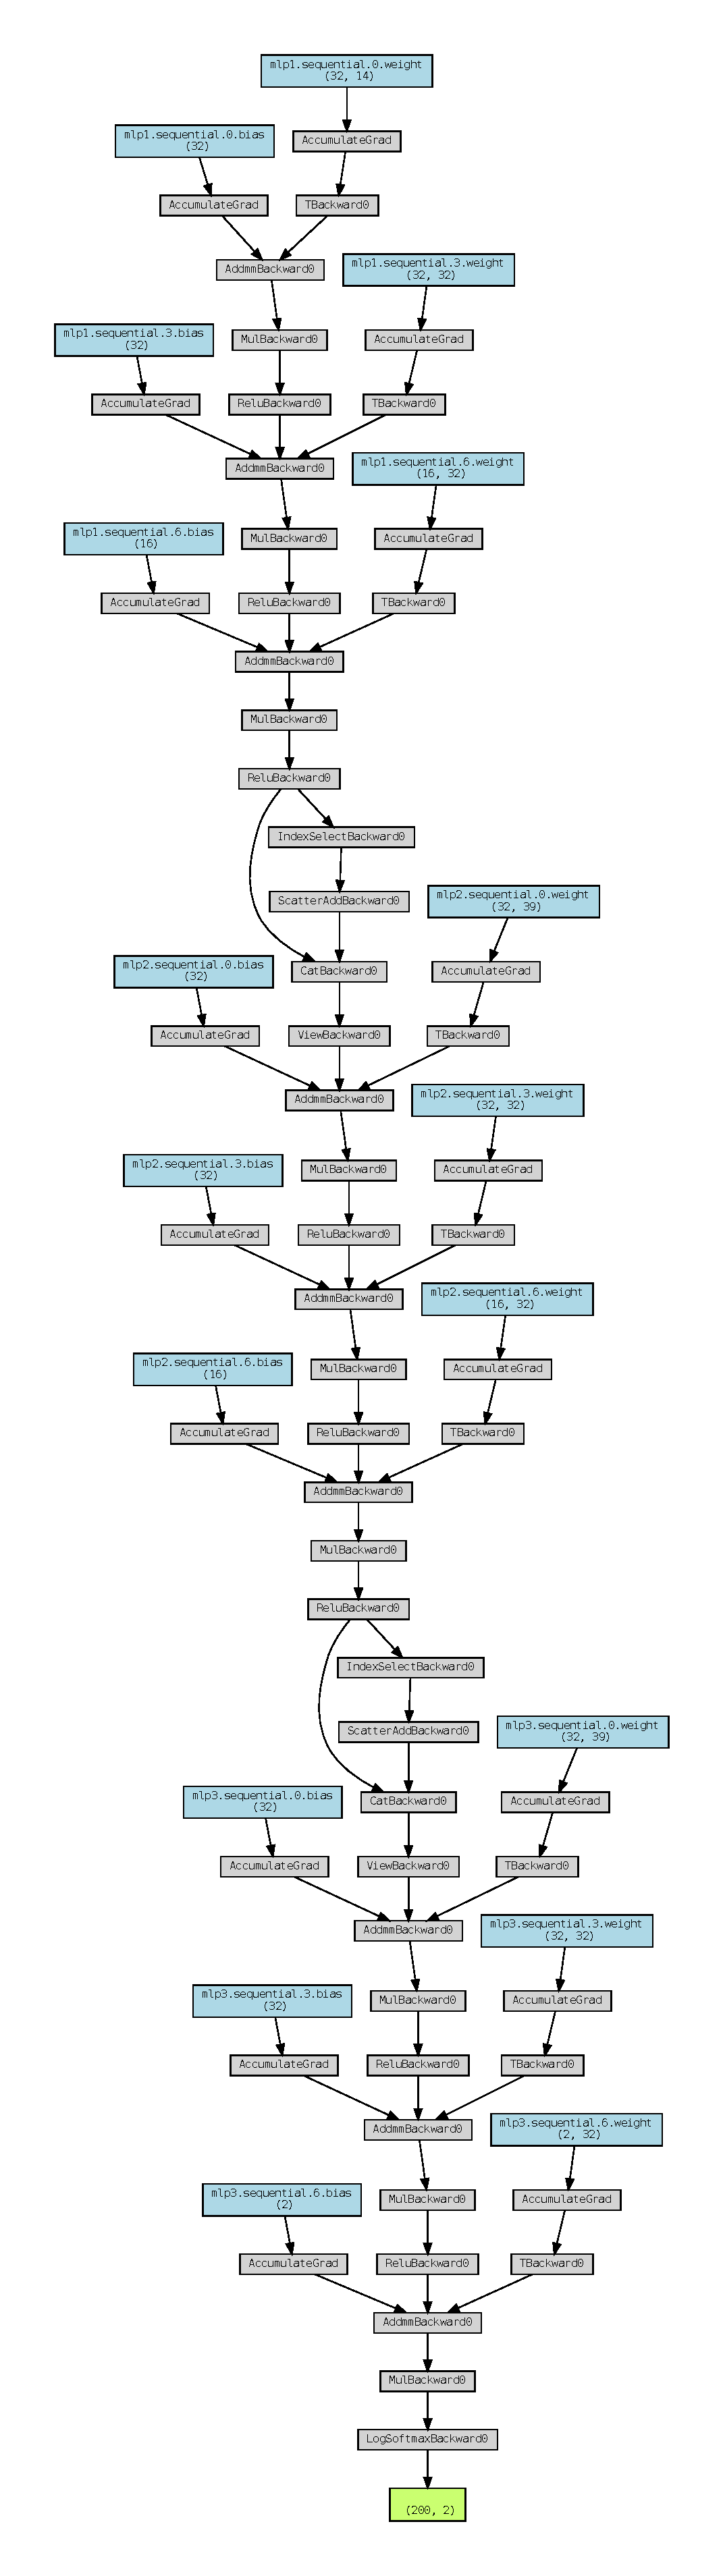
\includegraphics[height=0.7\paperheight]{figures/baseline_arch}
     \caption{Architecture for BASELINE.}
     \label{fig:baseline_arch}
\end{figure}

See \Cref{fig:baseline_arch} for a visualization.

\subsubsection{WMVC}
Next, we would like to experiment with more graph learning techniques
to develop the WMVC architecture.
Again,
it consists of three message passing layers
interwoven with 3-layer MLPs
as well as a random walk positional encoding.
In addition,
we include a Chebyshev convolution \citet{defferrard2016conv} before the message pasing layers,
which is a spectral graph convolution.
Moreover,
we also employ the GATv2 operator \citet{brody2021attentive} before the message passing layers,
which is a graph attention operator which fixes the static attention problem from its predecessor,
the graph attentional operator \citet{velivckovic2017graph}.
Finally,
WMVC employs multiple aggregation heads \citet{corso2020principal, tailor2021we} in its message passing layers which BASELINE lacks.

\begin{figure}
     \centering
     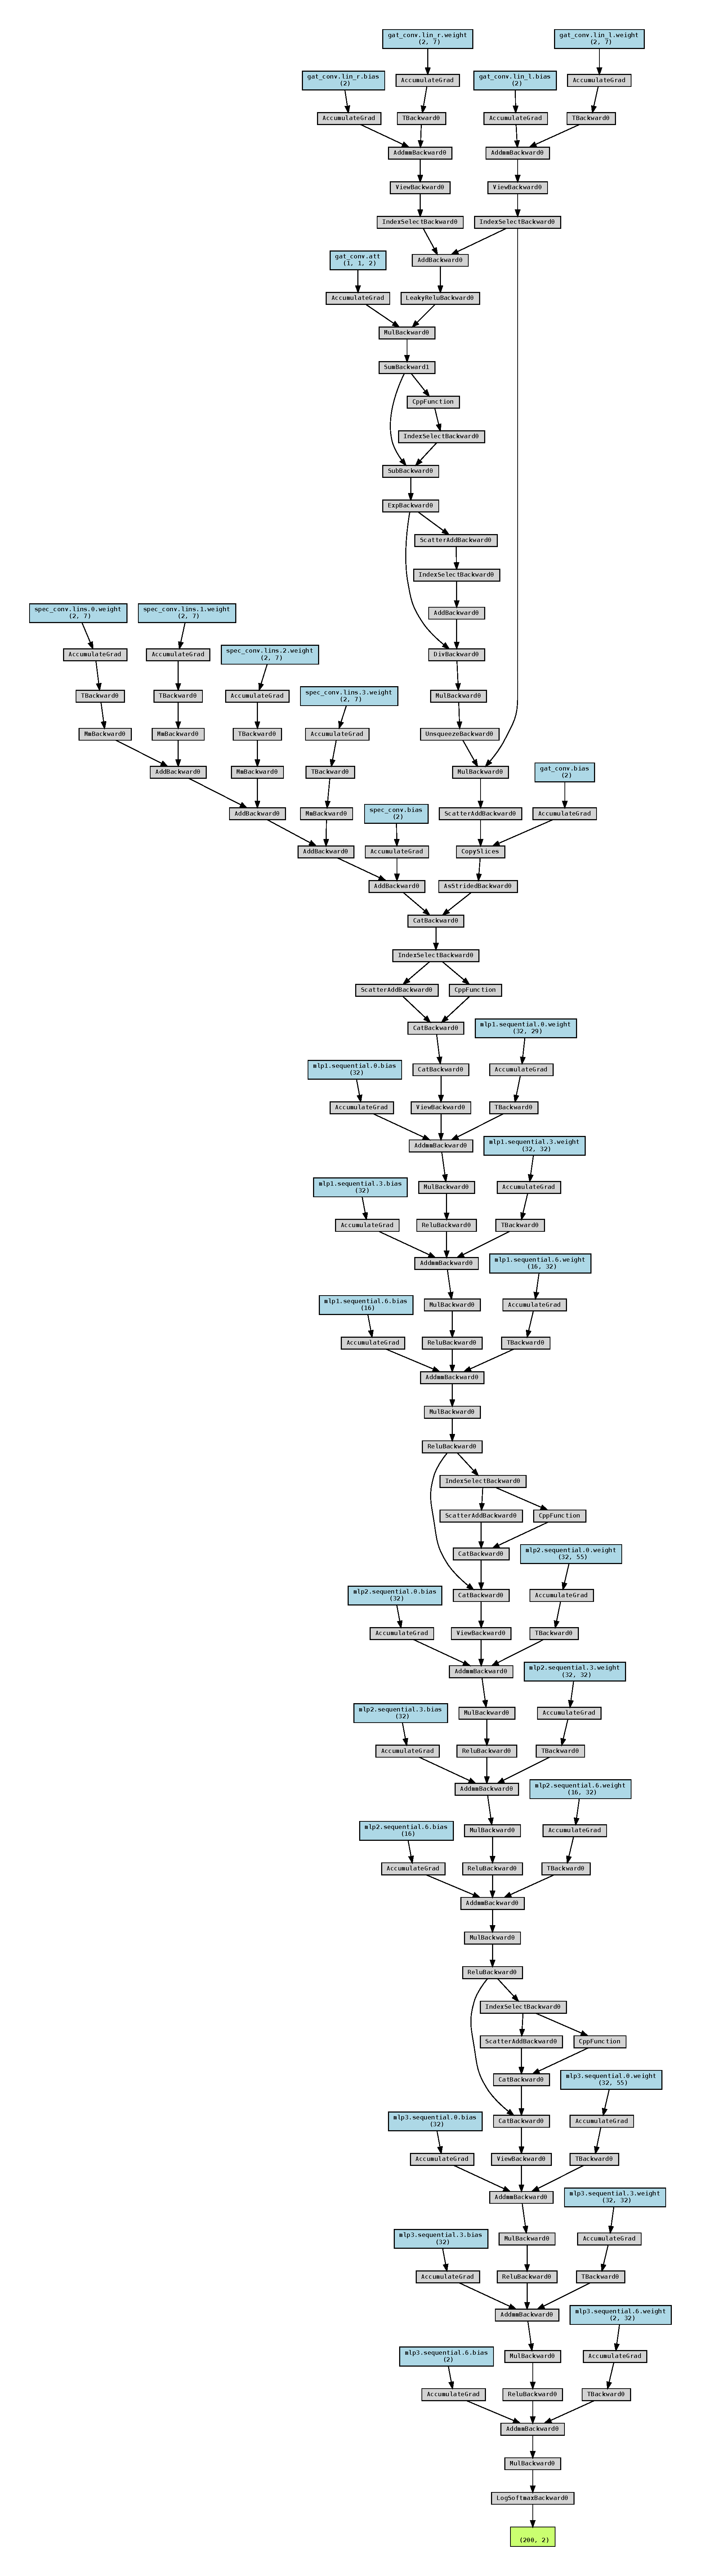
\includegraphics[height=0.7\paperheight]{figures/wmvc_arch}
     \caption{Architecture for WMVC.}
     \label{fig:wmvc_arch}
\end{figure}

See \Cref{fig:wmvc_arch} for a visualization.

\subsection{Iterating (Optional)}
Given the output from our GNN,
we can choose to include or exclude some vertices from the solution.
Then,
we can optionally attempt further reductions before computing a final solution.

\subsection{Computing a Final Solution}
If the current solution is not integral,
there is a simple greedy algorithm to ``round'' the solution to an independent set.
Namely, we sort the vertices in non-increasing fashion based on the outputted probabilities of our GNN.
Then, we greedily add the highest unprocessed vertex to our independent set
while marking all of its neighbors as not belonging to the set.

While this is the simplest method,
the greedy rounding algorithm is certainly not the only choice.
We can employ some sort of local search algorithm \citet{dahlum2016accelerating, chang2017computing} in place of the greedy algorithm we implemented.
Once again,
our implementation is geared towards simplicity
and a sufficiently fast local search implementation
should most likely be done using a compiled language.

\section{Experiments}
\subsection{Datasets}
We consider both real-world graphs and synthetic graphs.
Since these graphs do not come with weights,
we augment each instance with uniformly random integer weights within the interval $[1, N]$.
It is known that with probability at least $1-\frac nN$,
there is a unique solution to WMIS \citet{isolation}.
Thus we chose $N = 2n$ in hopes that this disambiguates supervised learning.

\subsection{PACE 2019 Graphs}
The PACE 2019 competition asked participants to solve MVC in 200 real-world graphs \citet{pace2019}.
Half of the dataset (odd indices) was provided to contestants
and the remaining half (even indices) was retained to evaluate submissions.
Solvers were given 30 minutes to solve each instance exactly.
The winning solution by \citet{wegotyoucovered} combined reduction rules,
local search, and a branch and bound scheme.

For each of the 200 PACE graphs,
we sampled 100 instances of uniform random vertex weights.
Out of the 20000 total instances,  
the state-of-the-art branch and reduce (B\&R) solver by \citet{kamis} solved 18197 cases within 6 hours.

\begin{figure}
     \centering
     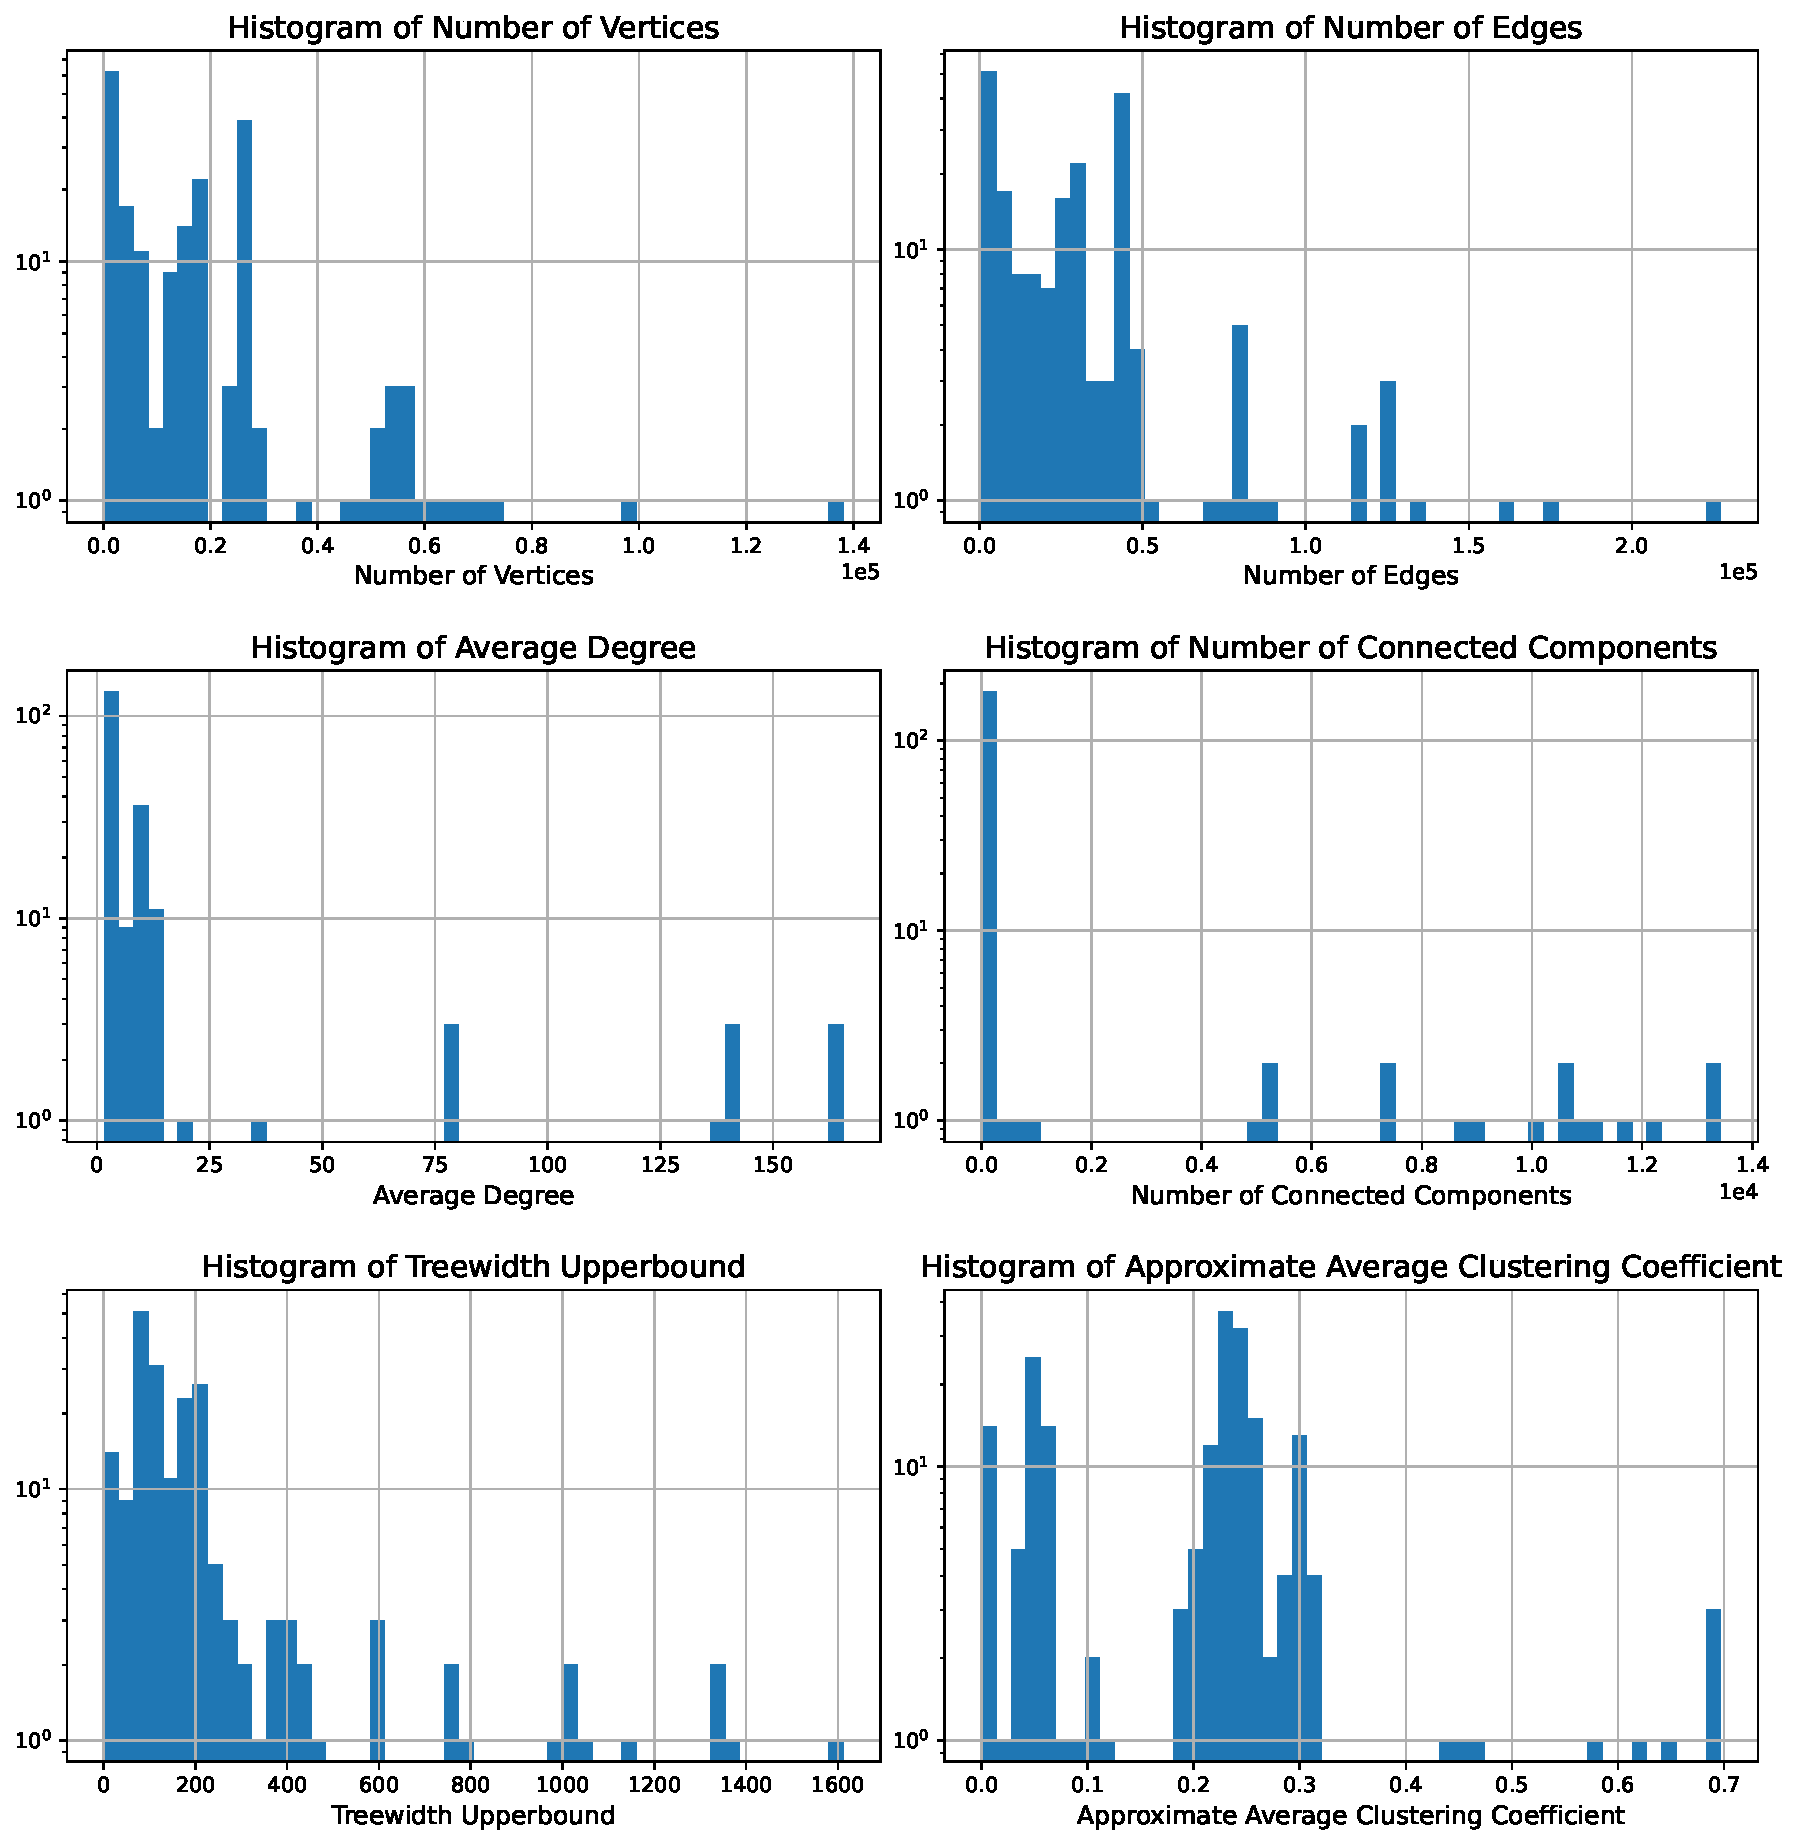
\includegraphics[width=\textwidth]{figures/pace_unweighted}
     \caption{Basic graph statistics as histograms for pace graphs.}
     \label{fig:pace_unweighted}
\end{figure}

See \Cref{fig:pace_unweighted} for some elementary statistics about the pace dataset.
It is interesting to note that this dataset is relatively sparse,
with mostly single digit average degree.
Moreover, most graphs have few connected components.

One trait of interest is how there is a bi-modal distribution for the \emph{approximate average clustering coefficient}.
The \emph{local clustering coefficient} of $v\in V$
is the fraction of triangles that exist over all possible triangles in $N(v)$.
The approximate average clustering coefficient
estimates the average of the local clustering coefficients across all nodes in a graph.
This suggests there are roughly two groups of PACE graphs in terms of the strength of community.

Informally speaking, \emph{treewidth} measures how far a graph is from being a tree \citet{robertson1986graph}.
Treewidth is a popular parameter in the parameterized complexity analysis of graph algorithms.
Many problems that are NP-hard for general graphs can be solved in polynomial time
with dynamic programming
when the treewidth is bounded by a constant.
Although treewidth is NP-hard to compute in general \citet{treewidth_hardness},
we compute an upperbound with heuristics based on node degrees \citet{bodlaender2010treewidth}.
We see that most PACE graphs have relatively small treewidth,
which may explain why most of them can be solved by B\&R.

\subsection{Erd\H os-R\'eyni Graphs}
We can generate an instance of an Erd\H os-R\'eyni graph $G(n, p)$ on $n$ vertices
by randomly connecting every pair of vertices independently
with some fixed probability $p$.

We generated 1000 instaces of $G(200, 0.1)$,
for which the B\&R solver by \citet{kamis} solved all cases within 6 hours.
Next, we generate 5000 instances of $G(1000, 0.005)$,
for which the B\&R solver solved 400 cases within 6 hours.
Finally, we generated 20000 instances of $G(50000, 0.00005)$.
for which the B\&R solver solved all cases within 6 hours.
It may be interesting to plot the fraction of cases solvable by B\&R
against the parameters $n, p$.

\begin{figure}
     \centering
     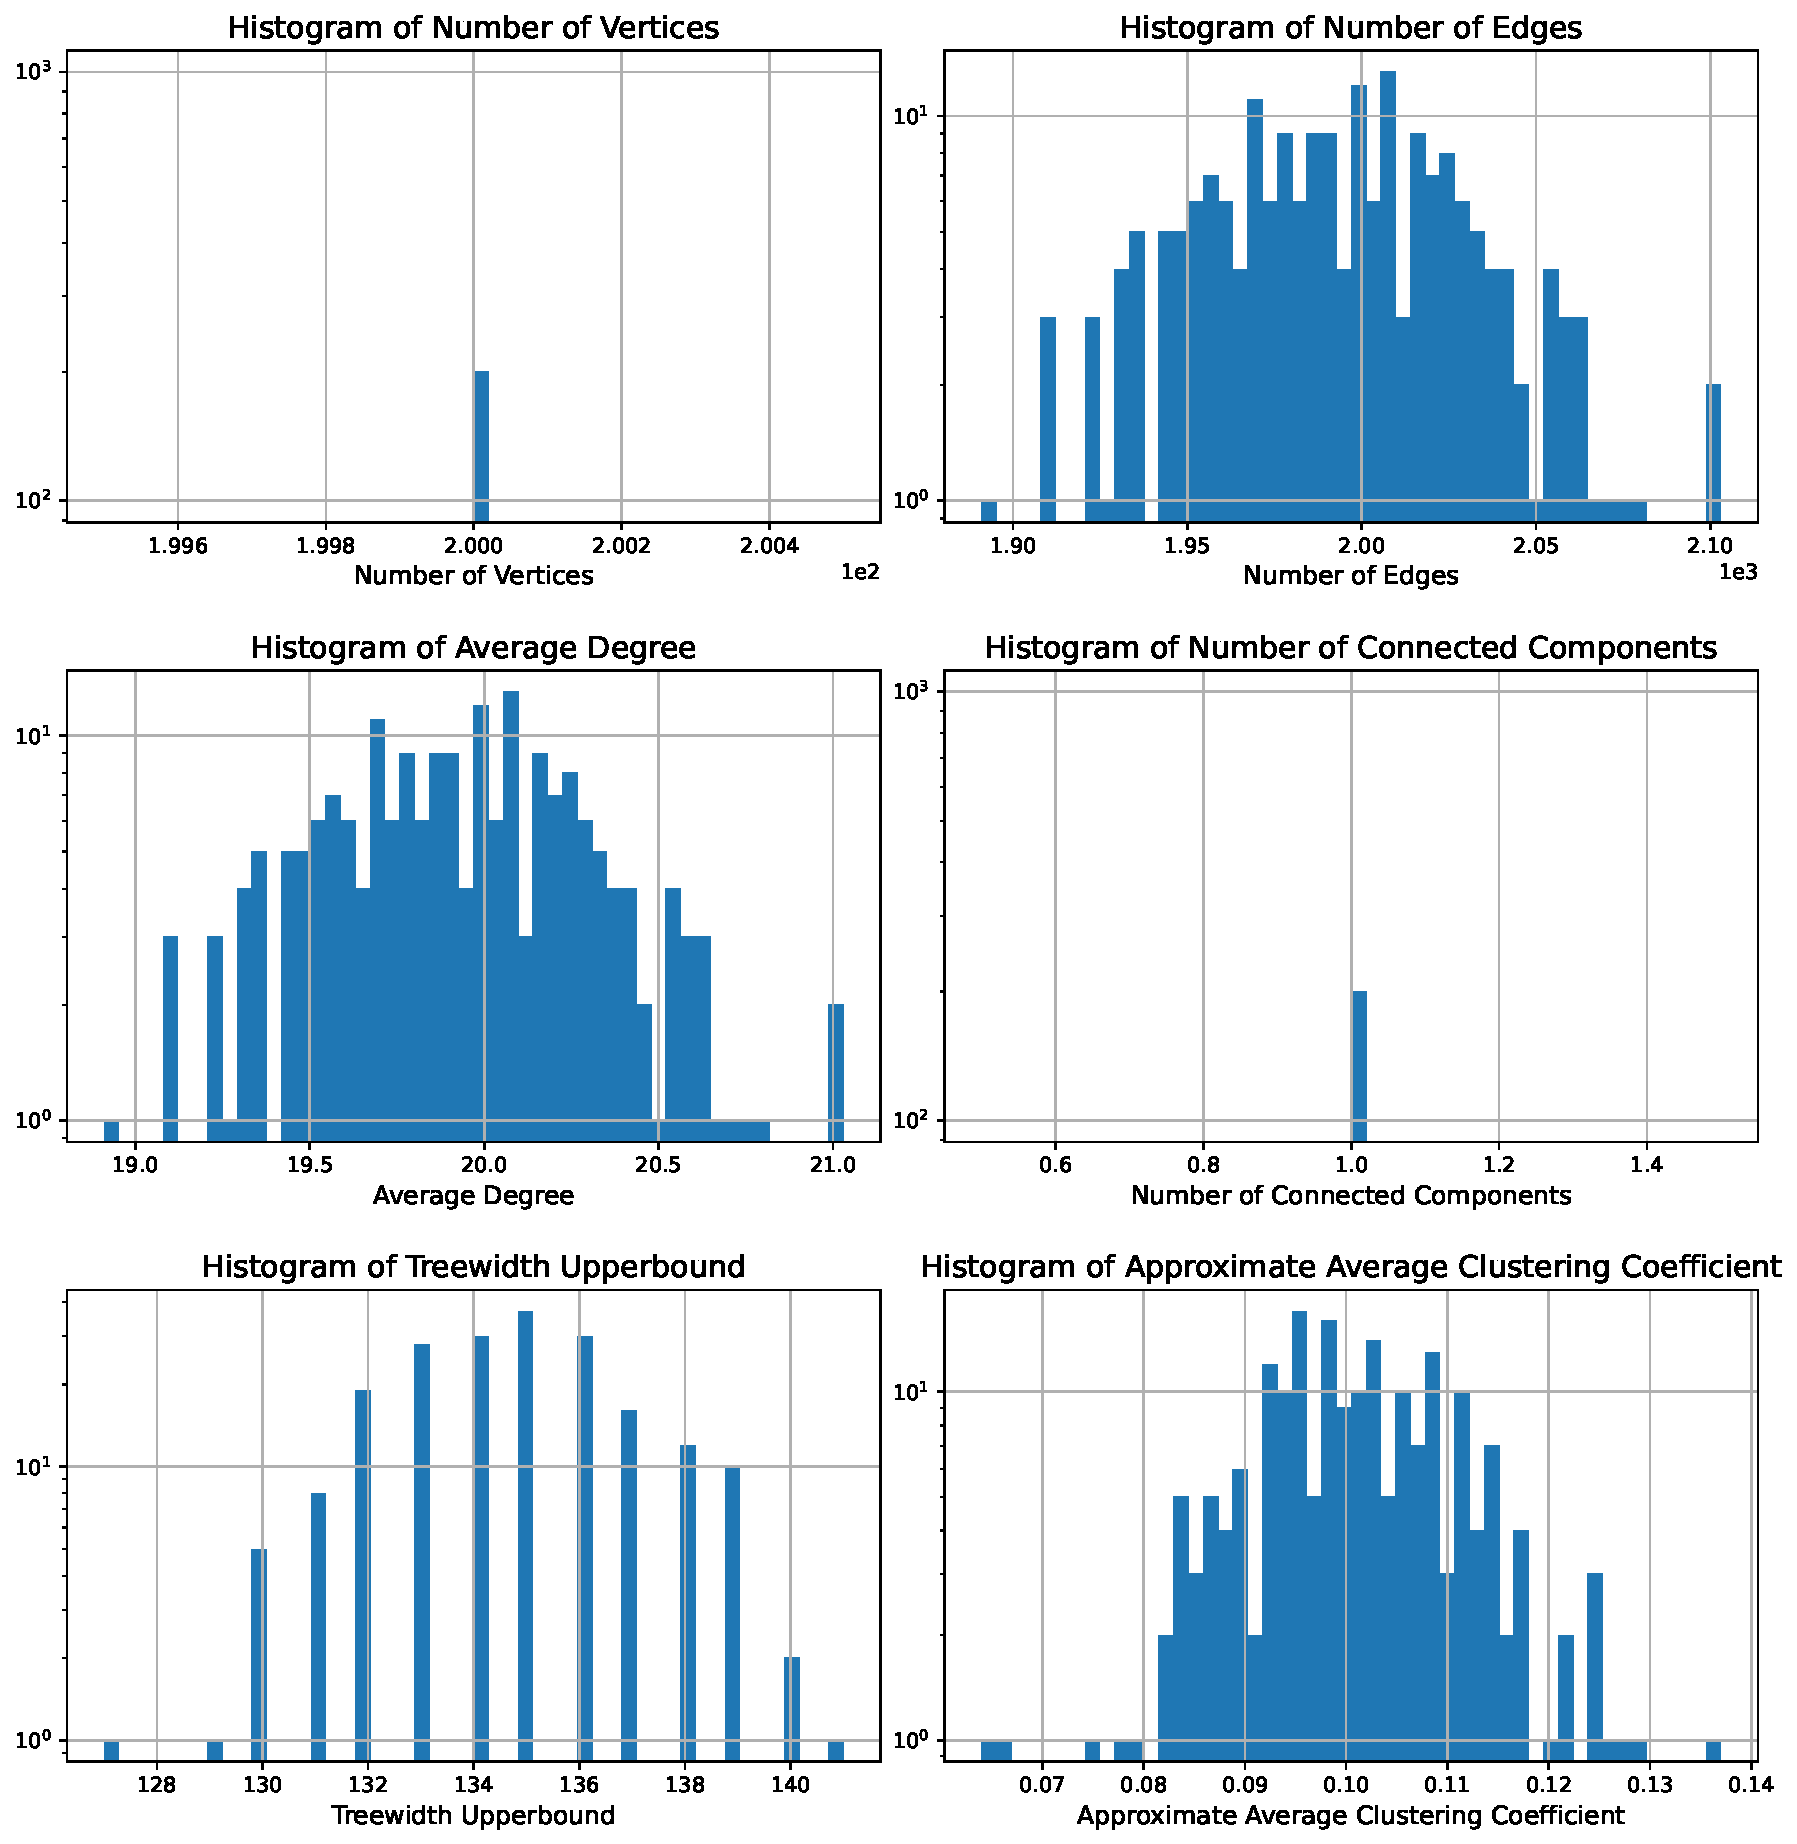
\includegraphics[width=\textwidth]{figures/erdos_reyni_small}
     \caption{Basic graph statistics as histograms for $G(200, 0.1)$ graphs.}
     \label{fig:erdos_reyni_small}
\end{figure}

See \Cref{fig:erdos_reyni_small} for some preliminary statistics of $G(200, 0.1)$,
computed from a sample of 200 from the 1000 generated instances.
As expected,
we see that the number of edges,
average degree,
treewidth upperbound,
and approximate average clustering coefficient
are all roughly normally distributed.

\subsection{Watts-Strogatz Graphs}
We also experiment with Watts-Strogatz graphs $G(n, k, p)$.
Also called ``small-world graphs'',
these graphs are generated by first taking a $k$-regular graph on $n$ vertices
and randomly rewiring each edge with probability $p$.

Specifically,
we generated 10000 instances of $G(1000, 5, 0.9)$.
Interestingly, for $k=5,6$,
the B\&R solver solved most cases within 6 hours.
However, for $k=7$, it fails to solve almost all the generated cases within 6 hours.
This may be due to the nature of the reduction rules,
some of which only work for very low degree vertices.

\subsection{Evaluation Metrics}
We would like to evaluate the performance of our framework on the PACE 2019 dataset \citet{pace2019},
Erd\H os-R\'eyni graphs,
and Watts-Strogatz graphs in two ways.
we would first like to look at the approximation ratio of our algorithm compared to the exact solutions
computed using B\&R \citet{kamis}.
Then, we would like to compare the approximation ratio of our algorithms compared to a heuristic local search
restricted to 30 minutes.
The second metric is necessary since the exact solver was unable to find the optimal result for about 10\% of PACE graphs
and more for the other datasets.

On all datasets,
we will reserve 20\% of the labeled dataset for evaluation
and the rest for training.

\subsection{Training Details}
For all datasets,
we used the SGD optimizer with a learning rate of 0.02 and momentum with parameter 0.9.
We trained for 300 epochs
and used a batch size of 256 graphs per batch.
We used negative loglikelihood loss
with class weights of 0.5 and 0.5 for the negative and positive examples,
respectively.
Finally,
we restricted ourselves to training on the graphs with at most 1000 nodes.
This amounts to fewer graphs per dataset,
especially for the PACE dataset.
However,
we will see that this still leads to decent approximatio ratios.

The evaluation metrics we employ for test set are accuracy,
accuracy 1,
and accuracy 10.
While accuracy is self-explanatory,
accuracy $k$ for some $k\in \N$ refers to the accuracy of the predictions for the $k$ highest ranked nodes.
That is,
the nodes for which the model is most confident belongs to a weighted maximum independent set.
This is more useful to us than raw accuracy
since our heuristic really only relies on the the most confident prediction(s).
\subsubsection{Features}
We employ node features in $\R^7$.
The first three features are the node weight,
the node degree,
and the sum of weights of neighbors.
The last four features are the random walk positional encodings
with total walk length 4.

\subsubsection{BASELINE}
For training the baseline model,
we attempted to replicate the hyperparameters of \citet{langedal_et_al}
as much as possible.
See \Cref{fig:baseline_test} for the training and test accuracy over the first 150 epochs.

\begin{figure}
     \centering
     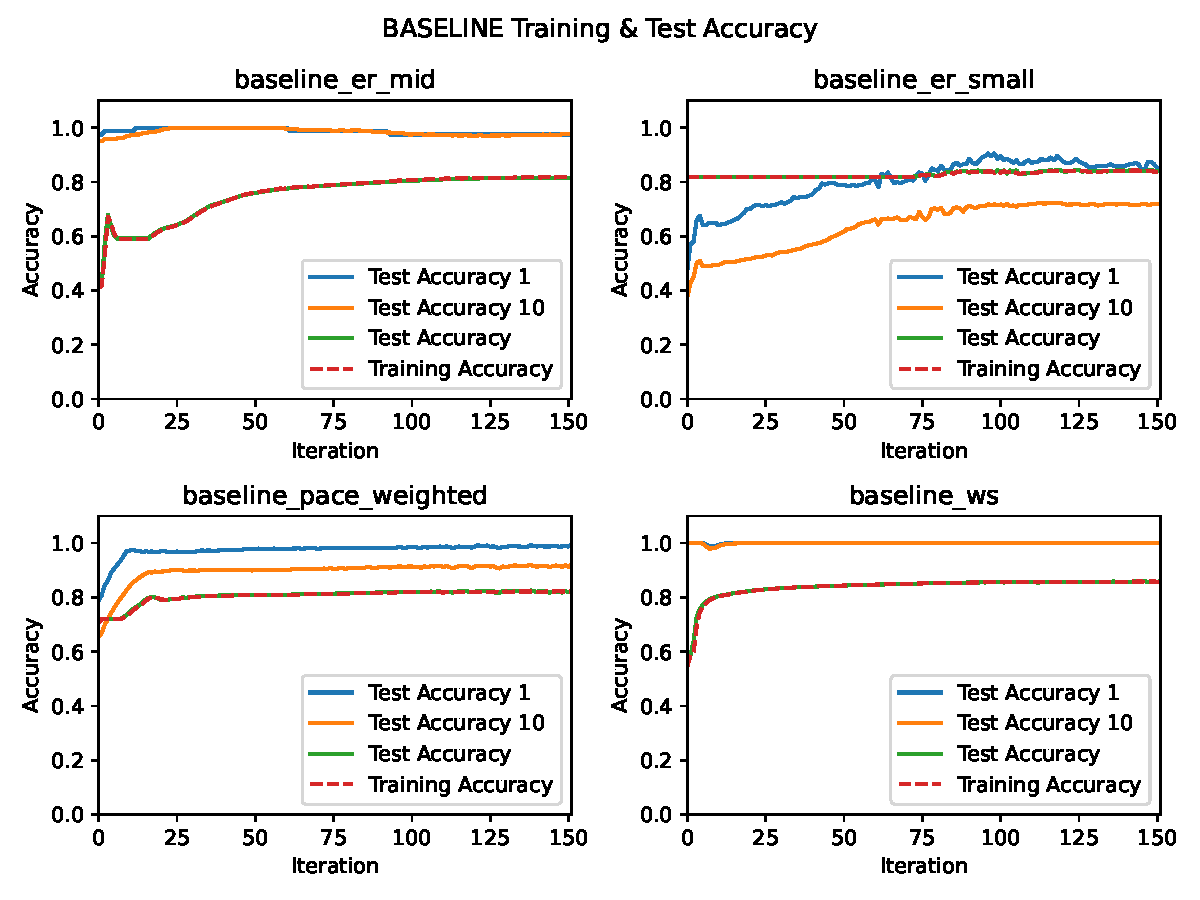
\includegraphics[width=\textwidth]{figures/baseline_test}
     \caption{BASELINE Train and Test Acuracy.}
     \label{fig:baseline_test}
\end{figure}

There are a few interesting observations we note here.
For one,
the accuracy 1 and accuracy 10 on the small Erd\H os-R\'eyni graphs
is lower than that of the mid-sized Erd\H os-R\'eyni graphs.
This may seem counterintuitive at first
but is reasonable since a smaller number of nodes means smaller number of nodes in a weighted maximum independent set.

We also note that the training and test accuracies are extremely similar
(but not the same when compared numerically).
This seems to suggest that our models are underfitting
and we can afford to introduce more expressiveness.

Another point of interest is the accuracy and accuracy $k$ on the Watts-Strogatz graphs.
This could be due to how every node has a very small number of neighbors
and hence there is less variance in neighborhood structure.

Finally,
we remark that even though accuracy plateaus rather quickly,
the accuracy $k$ metrics tend to increase as training progresses,
especially on the small Erd\H os-R\'eyni graphs.

\subsubsection{WMVC}
We had the exact same hyperparameters
when training the WMVC model
except for the class weights which are now 0.2 and 0.8
for the negative and positive examples,
respectively.
See \Cref{fig:wmvc_test} for the training and test accuracy over the first 150 epochs.

\begin{figure}
     \centering
     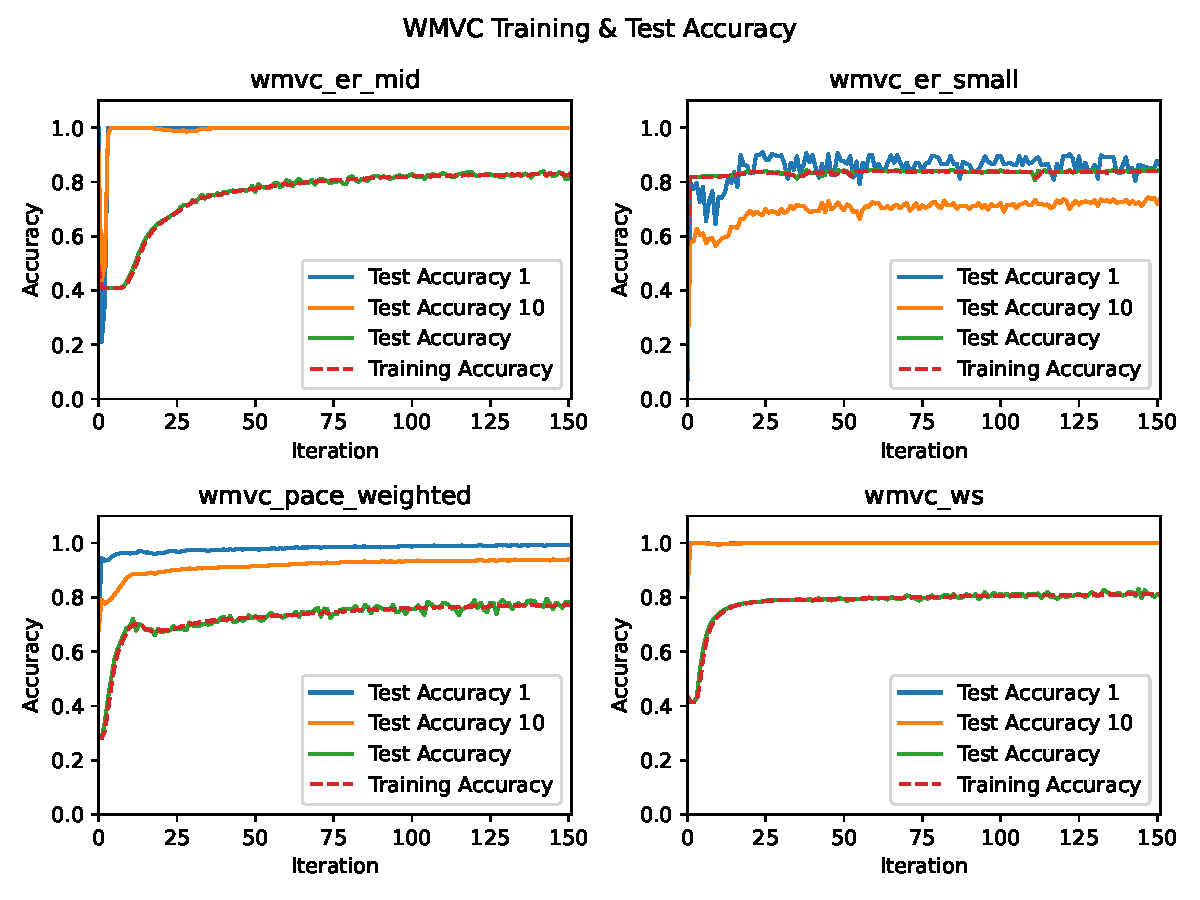
\includegraphics[width=\textwidth]{figures/wmvc_test}
     \caption{WMVC Train and Test Accuracy.}
     \label{fig:wmvc_test}
\end{figure}

We observe very similar patterns in training compared to the BASELINE model.
The only exception could be the greater fluctuation in the accuracy $k$ metric in the small Erd\H os-R\'eyni graphs.
A possible explanation could be that the learning rate should be decreased as training progresses.

\subsection{Results \& Analysis}
We compare the quality of weighted independent sets with two other algorithms.
One is the simple greedy algorithm which greedily chooses the unprocessed vertex with heaviest weight
to add to the solution.
The other algorithm we compare our models to is the sophisticated local search algorithm by \citet{kamis}.
It employs many complicated reduction rules
and performs well on many huge graphs.
We run each algorithm for a maximum of 30 minutes per graph,
which is significantly less than the 7 hours we allowed for the exact B\&R solver.
See \Cref{fig:approx_ratio} for the boxplots of approximation ratios on each dataset.
Note that we filtered by the graphs for which we were able to compute exact solutions.

\subsubsection{Approximation Ratio}
\begin{figure}
     \centering
     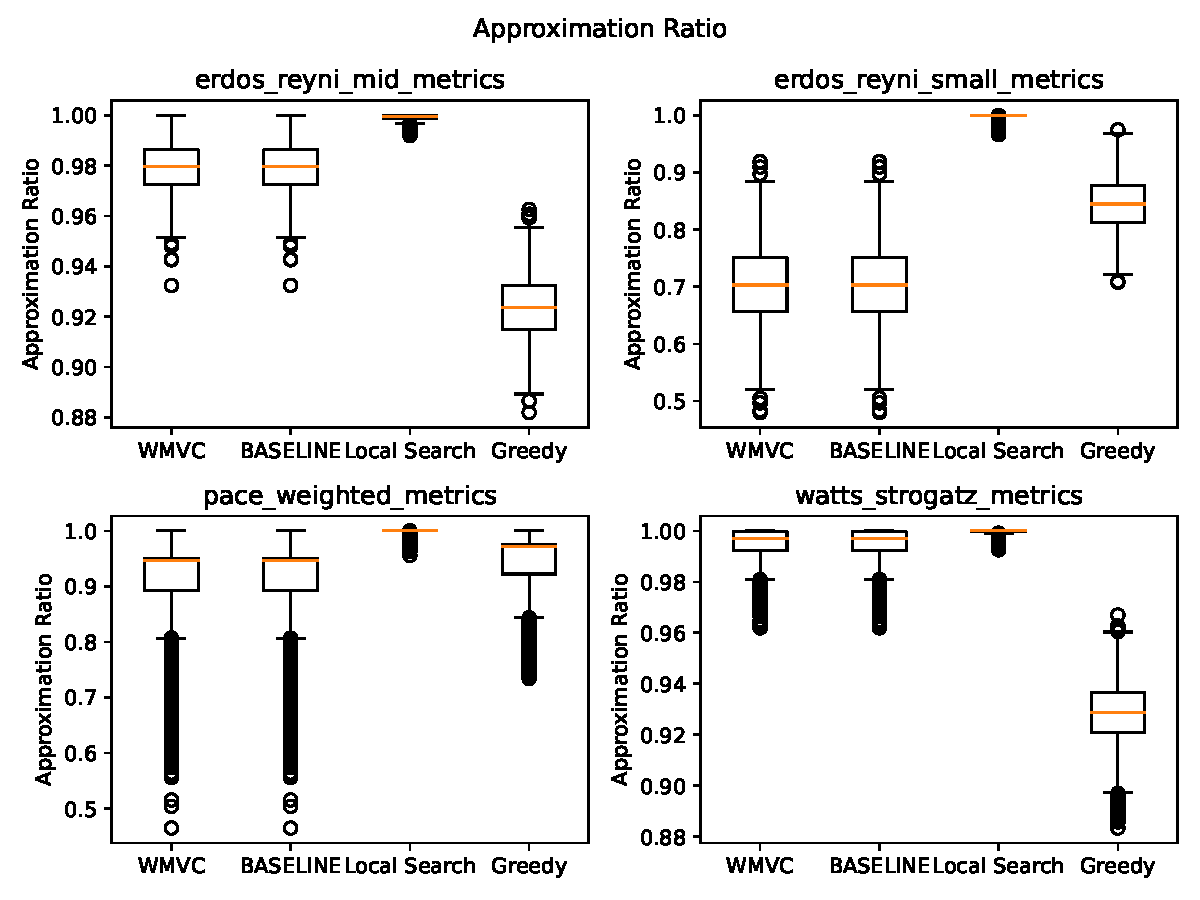
\includegraphics[width=\textwidth]{figures/approx_ratio}
     \caption{Approximation Ratio.}
     \label{fig:approx_ratio}
\end{figure}

The local search algorithm is very good.
It almost always finds a solution that is close to optimal,
save some small number of outliers.
We note that there could be some bias in data
since the exact B\&R solver shares some of the reduction rules with the local search algorithm.
Thus if the B\&R solver found an optimal solution,
it is likely that the local search algorithm can find a very good one at least.

Interestingly,
the greedy algorithm on the small Erd\H os-R\'eyni graphs actually outperforms both BASELINE and WMVC.
This could be due to the smaller number of total nodes,
which increases the difficulty of finding a node belonging to a weighted maximum independent set.
A possible improvement to our heuristic is to resort to the greedy algorithm once the number of unprocessed nodes falls below a threshold.

For the Watts-Strogatz graphs,
our models perform relatively better than the greedy heuristic.
The reason for which could be the same as the accuracy $k$:
every node has a very small number of neighbors
and hence there is less variance in neighborhood structure.

\subsubsection{Performance Ratio to Local Search}
Since the B\&R solver was not able to find an exact solution for every graph,
we compare the performance of our two models and the greedy algorithm
with the performance of the local search heuristic.
See \Cref{fig:local_search} for the ratios.

\begin{figure}
     \centering
     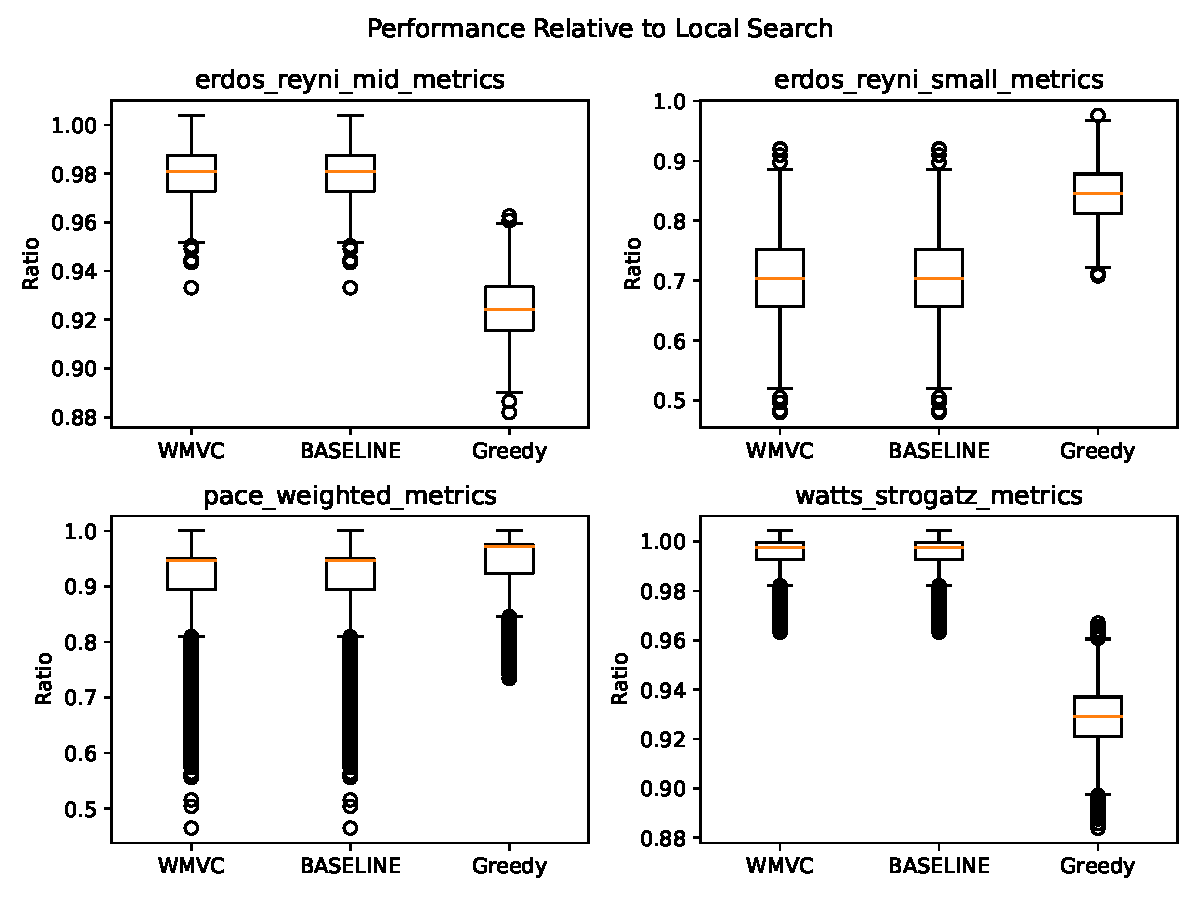
\includegraphics[width=\textwidth]{figures/local_search}
     \caption{Performance Relative to Local Search.}
     \label{fig:local_search}
\end{figure}

\section{Conclusion \& Future Work}\label{sec:conclusion}
We explored model improvements to the neural heuristic to solving WMIS by \citet{langedal_et_al}
as well as provided a simple,
extensible implementation of the heuristic.
We experimented on two random graph datasets
as well as a real life dataset.
In the future,
we hope to include more sophisticated preprocessing and postprocessing steps,
as well as improve the GNN architecture to yield improved heuristics.
One promising direction for developing better GNN architectures
is to bypass the need for node labels
and directly train our models on the (possibly adjusted) objective function of interest \citet{karalias2022neural}.

\section{References}
\bibliographystyle{plainnat}
\bibliography{report.bib}


\end{document}
